\begin{answer}

\centering
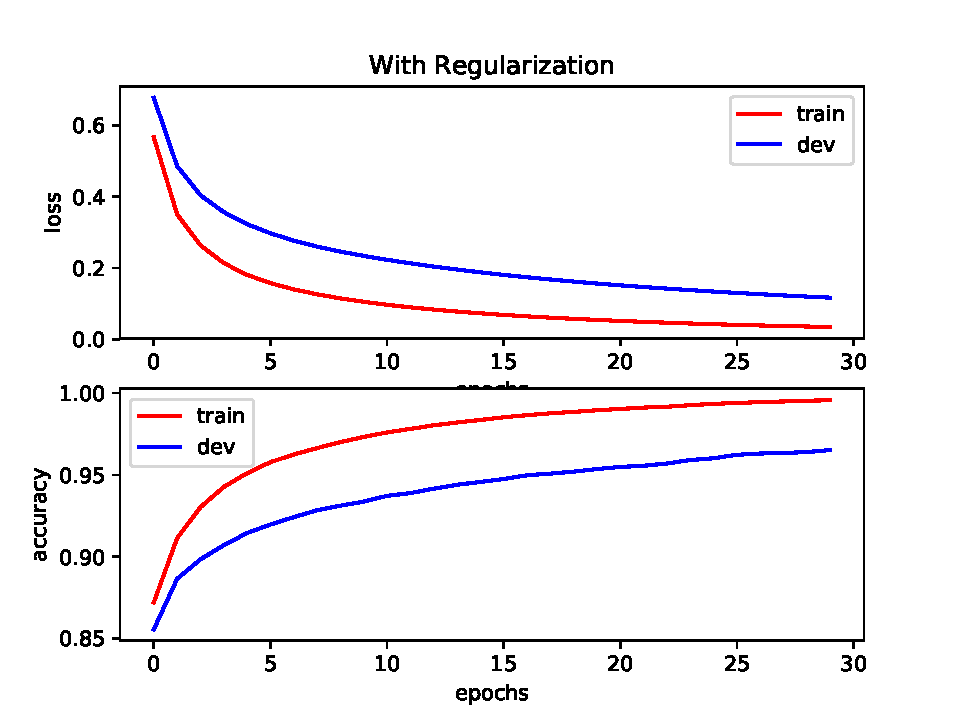
\includegraphics[width=6in]{regularized.pdf} 
REGULARIZED model



There is a clear change in loss and accuracy between baseline and regularization plots.
The train set:
Is similar in accuracy and loss for both models, as the model attempts to fit the training data and reduce bias.
For dev set:
In the baseline model both loss and accuracy become stagnant after around 8 epochs. Loss reaches minimum at around 0.4 and accuracy reaches max on 0.92.
The regularized model however, causes the model to continue increasing accuracy and reducing loss after 8 epochs.
We see that even after 25 epochs, accuracy is reaching 0.95 and loss is going down to 0.2

The comparison from both plots shows how regularization has caused the model to penalize the model from overfitting the training set, by reducing variance. The dev set is getting a better approximation in accuracy and reduction of loss.

   
\end{answer}
   